%-------------------------------------------------------------
\documentclass{beamer}
\usepackage[utf8]{inputenc}
\usepackage{hyperref}
\usepackage[T1]{fontenc}
\usepackage{tikz}

\usepackage{latexsym,xcolor,multicol,booktabs,calligra}
\usepackage{amsmath,amssymb,BOONDOX-cal,bm}	
\usepackage{graphicx,pstricks,stackengine}      
%bibliography
\usepackage[numbers]{natbib}
%reference: https://tex.stackexchange.com/questions/202963/how-to-cite-author-in-ieee-format
%The natbib package provides three versions of the standard BibTeX bibliography styles compatible with author-year citations (\citet, \citeauthor, \citeyear):
%1.plainnat
%2.bbrvnat
%3.unsrtnat

\author{Qitong Cao}
%\titlegraphic{\includegraphics[width=\textwidth]{unilogo4cmittel.jpg}}
\titlegraphic{ 
\begin{tikzpicture}[overlay,remember picture]
\node[right=-0.15cm] at (current page.150){
    
\includegraphics[width=0.2\textwidth]{cropped-cropped-big_Duke-Kunshan-University-Logo.png}
};
\end{tikzpicture}
}
\title{"Voting-Based Decentralized Consensus Design for Improving the Efficiency and Security of Consortium Blockchain"}
\institute{Duke Kunshan University \\ CS/Econ 206 | Computational Economics } 
\date{May 5 2022}
%\logo{\includegraphics[width=0.12\textwidth]{MessmapLogo.png}}

\usepackage{Wue}

\def\cmd#1{\texttt{\color{red}\footnotesize $\backslash$#1}}
\def\env#1{\texttt{\color{blue}\footnotesize #1}}

\newtheorem{thm}{Theorem}[theorem]


%—-------------------------------------------------------------

\begin{document}
	\begin{frame}
    \titlepage
    \end{frame}

	
	\begin{frame}
		\tableofcontents[sectionstyle=show,subsectionstyle=show/shaded/hide,subsubsectionstyle=show/shaded/hide]
	\end{frame}
		
	
	%—------------------------------------------------------
	\section{Part I: Summary}
	    %\subsection{}
	    
	    \begin{frame}{1.Background and Motivation}
 
		\begin{columns}[T]
			\begin{column}<0->{.5\textwidth}
				\begin{figure}[thpb]
					\centering
					\resizebox{1.2\linewidth}{!}{
						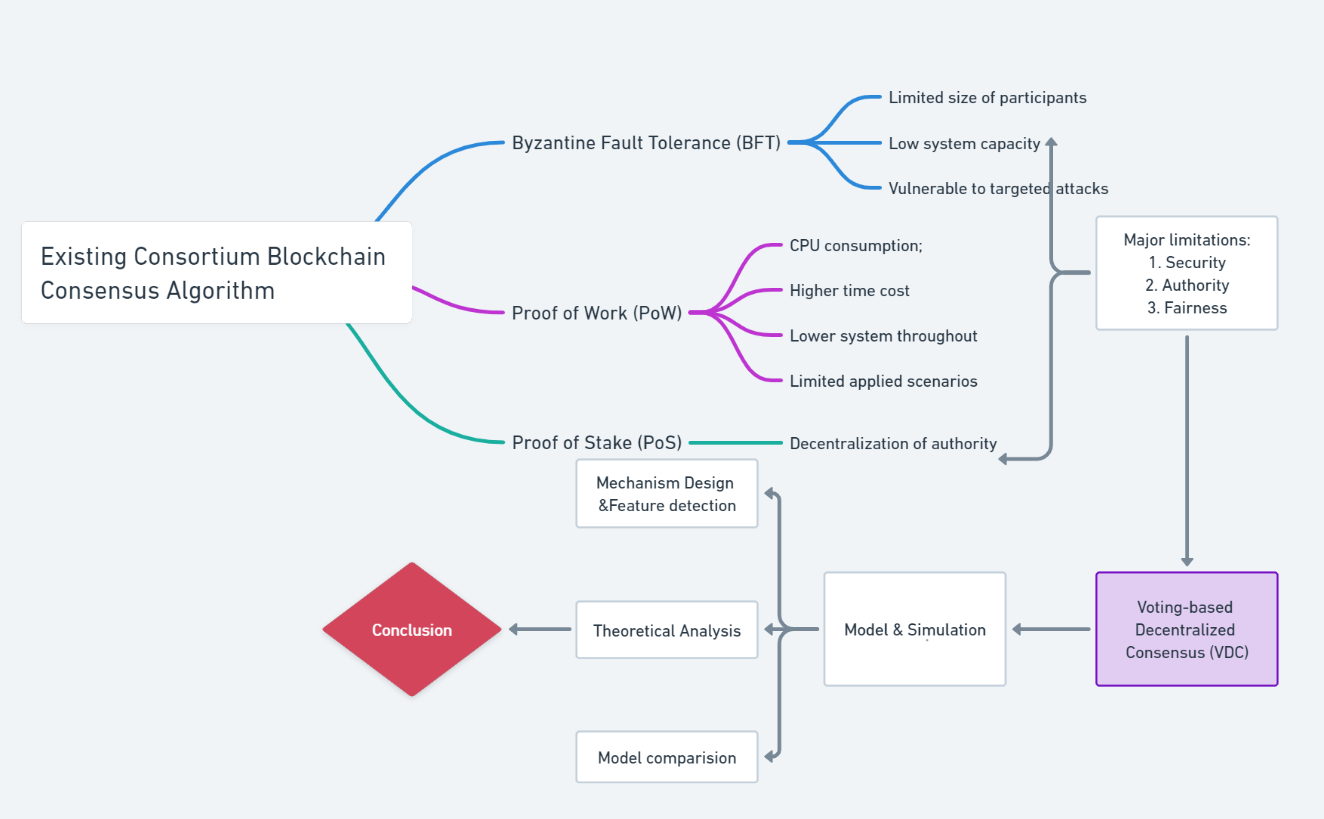
\includegraphics{mindmap.png}
					}
					%	\includegraphics[scale=1.0]{figurefile}
					\caption{Summary Mindmap created by Whimsical}
					\label{fig:1}
				\end{figure}
			\end{column}%
			\hfill%
			\begin{column}<0->{.5\textwidth}
				\begin{itemize}
					\item<1-> Background
					\begin{itemize}
						\item<1-> Limitations: high energy consumption, time inefficiency, low transaction throughput, poor security, poor user revenue fairness (Sun et al. 2020).
					\end{itemize}
					\item<2-> Motivation
					\begin{itemize}
						\item<2-> To  improve the efficiency and security of the consortium blockchain to and the performance of the blockchain platform.
					\end{itemize}
				\end{itemize}
			\end{column}
		\end{columns}
	\end{frame}
		    \begin{frame}{Research Question}
			    \begin{itemize} 
			    \item  Research Questions: How to improve the efficiency and security of consortium blockchain?
			    \end{itemize}
		    \end{frame}
		\begin{frame}[fragile]{Methods}
		\begin{exampleblock}{Model \& Simulation method}
			\centering
			\footnotesize
			\begin{itemize}
			    \item Authority: by increasing uncertainty
			     \item Security: by introducing "lottery drawing" to avoid attacks
			     \item Regulation: by adding "asset" to increase "crime cost"
			\end{itemize}{ll}
			
		\end{exampleblock}
		\begin{exampleblock}{Model Comparison}
			\centering
			\footnotesize
			\begin{itemize}
			    \item Compare with Practical Byzantine Fault Tolerance (PBFT) and Mixed Byzantine Fault Tolerance (MBFT) algorithms
			    \item shows apparent advantages in user benefit fairness, time efficiency, and elasticity against target attack and has acceptable extra cost in energy consumption.
			\end{itemize}
				
		\end{exampleblock}
	\end{frame}
	
		\begin{frame}{ Intellectual Merits}
		 \begin{block}{Proof of Work (PoW)}<1->
		   the cost of additional CPU consumption; higher time cost; lower system throughput;the quality of service requirements of some scenarios (Frankenfield 2021).
		   \begin{itemize}
		       \item increase the cost of malicious behavior
		   \end{itemize}
		 \end{block}
	       
		\begin{block}{ Proof of Stake (PoS)}<2->
            the decentralization of authority
            \begin{itemize}
                \item converted identities to limit and disperse authority to avoid monopoly
            \end{itemize}
        \end{block}
    	
		\begin{block}{Byzantine Fault Tolerance (BFT) algorithm}<3->
		  low system capacity; leaders vulnerable to targeted attacks  
		  \begin{itemize}
		       \item utilize the  unpredictability against the targeted attacks
		   \end{itemize}
		\end{block}
       
	\end{frame}
	
	\begin{frame}{Practical Impacts}
			    \begin{itemize} 
			    \item  The new consensus algorithm is expected to solve the drawbacks of the existing blockchain algorithms or update the current consensus algorithm to improve the performance of the blockchain platform. 
			    \item As a newly born partial theoretical algorithm mechanism, VDC also needs further experiments and improvements to adapt to highly complex application scenarios (Sun et al. 2020).
			    \end{itemize}
		    \end{frame}
	%-------------------------------------------------------
	
	
	
	
	
	
	
	
	
	
	
	\section{Part II: Critics}
	    %\subsection{}
			   
		    \begin{frame}{Critics}
 
		\begin{columns}[T]
			\begin{column}<0->{.5\textwidth}
				\begin{figure}[thpb]
					\centering
					\resizebox{1.2\linewidth}{!}{
						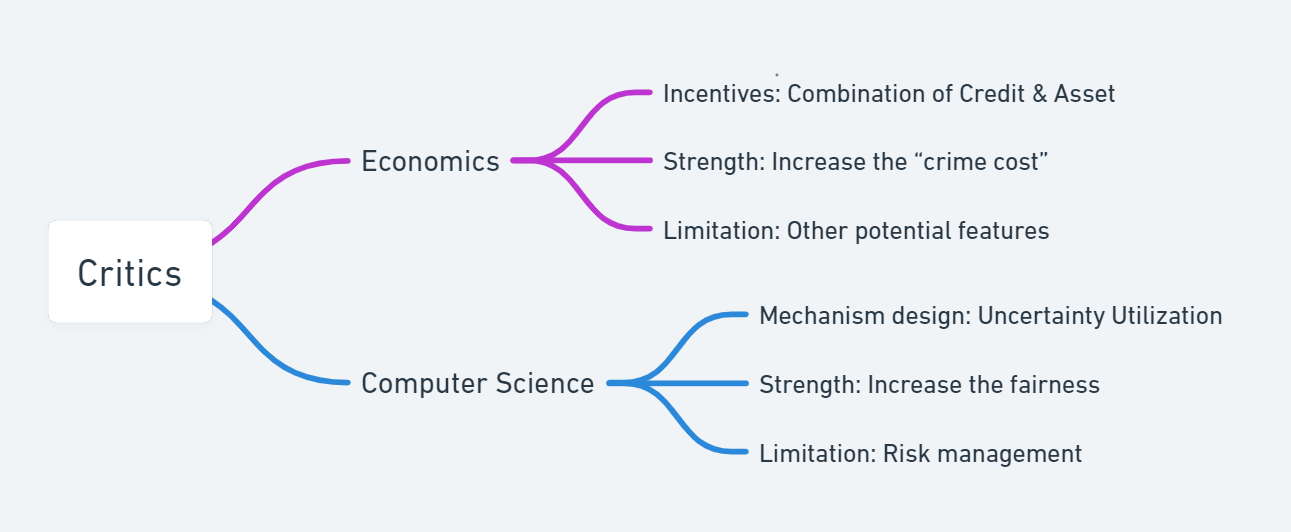
\includegraphics{mindmap2.png}
					}
					%	\includegraphics[scale=1.0]{figurefile}
					\caption{Critics Mindmap created by Whimsical}
					\label{fig:1}
				\end{figure}
			\end{column}%
			\hfill%
			\begin{column}<0->{.5\textwidth}
				\begin{itemize}
					\item<1-> Economics for Computer Science
					\begin{itemize}
						\item<1-> Incentives: Combination of Credit \& Asset
				\item<1-> Strength: Increase the "crime cost"
				\item<1-> Limitation: Other potential features	\end{itemize}
					\item<2->  Computer Science for Economics
					\begin{itemize}
						\item<2-> Mechanism design: Uncertainty Utilization
							\item<2->Strength: Increase the fairness
								\item<2->Limitation: Risk Management
					\end{itemize}
				\end{itemize}
			\end{column}
		\end{columns}
	\end{frame}		   
			   
			   
			   
			   
		
	%-----------------------------------------------------
	\section{Part III: Inspirations}
	    %\subsection{}

 \begin{frame}{Inspirations}
 
		\begin{columns}[T]
			\begin{column}<0->{.5\textwidth}
				\begin{figure}[thpb]
					\centering
					\resizebox{1.2\linewidth}{!}{
						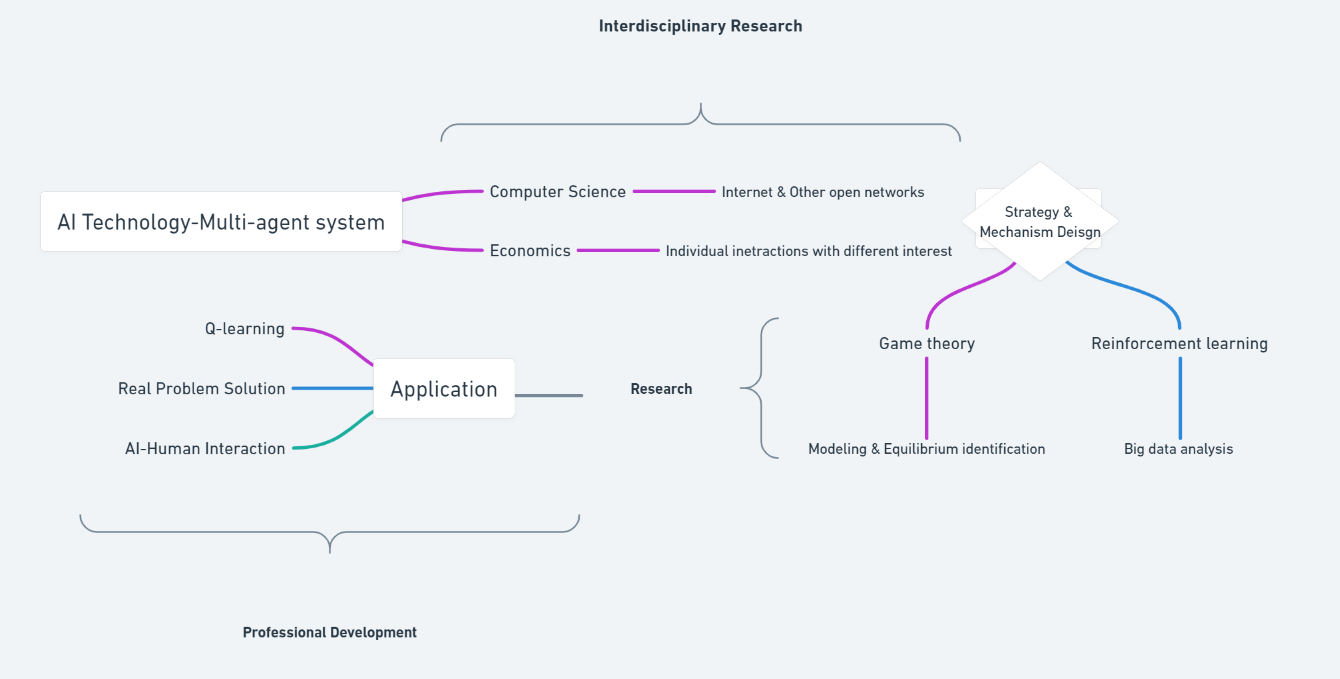
\includegraphics{mindmap3.png}
					}
					%	\includegraphics[scale=1.0]{figurefile}
					\caption{Inspirations Mindmap created by Whimsical}
					\label{fig:1}
				\end{figure}
			\end{column}%
			\hfill%
			\begin{column}<0->{.5\textwidth}
				\begin{itemize}
				\item<1-> Interdisciplinary Research
			\begin{itemize}
			    \item <1-> Interactions with other non-human agents
			\end{itemize}	\item<2->Research for Real-world Practices
			\begin{itemize}
			    \item<2-> Game Theory Model Construction
			    \item<2->Reinforcement learning with big data
			\end{itemize}	\item<3->Future Professional Growth
			\begin{itemize}
			    \item Applications: content ranking in user-generated content sites
			\end{itemize}
					\end{itemize}
			\end{column}
		\end{columns}
	\end{frame}	


	%-------------------------------------------------
    	\section{References}		\begin{frame}{Revision responding to peer review}
		\begin{itemize}
			\item Jargon Explanation
			\begin{itemize}
				\item Definition of technical words added to the article
				\item Glossary table of major words construction
				\item Abbreviations spelled out 
			\end{itemize}
			\item More citations
			\begin{itemize}
				\item Citations of major technical words
				\item Citations in "Background" and "Intellectual Merits"  
			\end{itemize}
			\item Revision of "Professional Development"
			\begin{itemize}
				\item Original part moved to Part II
				\item More related topic added  
			\end{itemize}
		\end{itemize}
		
	\end{frame}
	
	\begin{frame}{Bibliography (Major Reference)}
		\begin{itemize}
			\item Website
			\begin{itemize}
				\item  “Consortium Blockchain | CoinMarketCap.” n.d. CoinMarketCap Alexandria. Accessed May 5, 2022.
				\item Frankenfield, Jake. 2019a. “Consensus Mechanism (Cryptocurrency).” Investopedia. 2019.
				\item “Practical Byzantine Fault Tolerance (PBFT) - BitcoinWiki.” n.d. En.bitcoinwiki.org. Accessed May 5, 2022.
			\end{itemize}
			\item Articles
			\begin{itemize}
				\item Dafoe, Allan, Yoram Bachrach, Gillian Hadfield, Eric Horvitz, Kate Larson, and Thore Graepel. 2021. “Cooperative AI: Machines Must Learn to Find Common Ground.” Nature 593 (7857): 33–36.
				\item Daly, Lyle. 2021. “What Is Byzantine Fault Tolerance?” The Motley Fool. November 10, 2021.
				\item Daly, Lyle. 2021. “What Is Byzantine Fault Tolerance?” The Motley Fool. November 10, 2021.
		\item Du,Mingxiao, Qijun Chen, and Xiaofeng Ma. 2020. “MBFT: A New Consensus Algorithm for Consortium Blockchain.” IEEE Access 8: 87665–75.	\end{itemize}
		\end{itemize}
		
	\end{frame}
\bibliographystyle{IEEEtranN}
\bibliography{Bibliography}
	%----------------------------------------------
%	\section{References}
%		
%		\begin{frame}[allowframebreaks]
%			\bibliographystyle{unsrt}
%			\bibliography{Bibliography.bib}	
%		\end{frame}
%%
	%-------------------------------------------
%	\begin{frame}
%		\begin{center}
%			{\Huge \emph {\textrm{Thank  ~you!}}}
%		\end{center}
%	\end{frame}

\end{document}